\documentclass{article}

\usepackage{float}
\usepackage[english]{babel}
\usepackage[a4paper,top=2cm,bottom=2cm,left=2cm,right=2cm,marginparwidth=1.75cm]{geometry}
\usepackage{amsmath, amssymb, amsthm}
\usepackage{graphicx}
\usepackage{subcaption} % Pour les sous-figures
\usepackage[colorlinks=true, allcolors=blue]{hyperref}
\usepackage{tikz}
\usetikzlibrary{arrows.meta}
\usepackage{array}
\usepackage{amssymb}
\usepackage{tcolorbox}
\usepackage{mdframed}
\usepackage{listings}
\usepackage{enumitem}


% Environnement de preuve personnalisé
\newmdenv[
  topline=false,
  bottomline=false,
  rightline=false,
  leftline=true,
  linecolor=gray,
  linewidth=1pt,
  skipabove=\baselineskip,
  skipbelow=\baselineskip,
  innerleftmargin=5pt,
  innerrightmargin=5pt,
  innertopmargin=5pt,
  innerbottommargin=5pt
]{proofbox}

\newenvironment{myproof}[1][\proofname]{%
  \begin{proofbox}%
}{\hfill$\qed$\end{proofbox}}


% Environnement Definition personnalisé
\newmdenv[
  topline=false,
  bottomline=true,
  rightline=false,
  leftline=true,
  linecolor=gray,
  linewidth=1pt,
  skipabove=\baselineskip,
  skipbelow=\baselineskip,
  innerleftmargin=5pt,
  innerrightmargin=5pt,
  innertopmargin=5pt,
  innerbottommargin=5pt
]{definitionbox}

\newenvironment{mydefinition}[1]{%
  \begin{definitionbox}%
  \noindent\textbf{#1}\par
}{%
  \end{definitionbox}%
}



\title{Compression d'images avec pertes}
\author{Maximilien Dubus, Candidat n°16078}
\date{2025}




\begin{document}
\maketitle


\section{Introduction}

Chaque jour 100 millions de photos sont publiées sur Instagram. En ne supposant aucune compression, cette plateforme doit stocker une estimation de 600 To en plus chaque jour.
En effet,    
\[
        \underbrace{100\,000\,000}_{\shortstack{\text{nombre de}\\\text{photos}}}
        \times
        \underbrace{2\,000 \times 1\,000}_{\shortstack{\text{\small nombre de}\\\text{pixels par photo}}}
        \times
        \underbrace{3}_{\shortstack{\text{nombre d'octets}\\\text{par pixel}}}
        =  600\ \text{To}
\]

Il est donc primordial d'utiliser une technique de compression qui exploite la redondance de l’information afin de réduire ces 600 To. De plus, il est possible d'utiliser une compression avec pertes, où la suppression de certaines informations permet de rendre le fichier encore moins volumineux. Il faut cependant bien choisir les informations à supprimer pour que l’image ne paraisse pas dégradée. Pour cela, on peut exploiter certaines limites physiologiques de l’œil humain.

Dans ce rapport, on s’intéresse à la compression JPEG, définie en 1991 par le groupe éponyme (JPEG: Joint Photographic Experts Group) et encore grandement utilisée aujourd'hui. L'objectif est d'analyser les performances en taille et en qualité de la compression JPEG afin d'élaborer une technique pour choisir le facteur de quantification le plus adapté à chaque image.

\section{Les étapes de la compression JPEG}

La compression JPEG est composée de six étapes principales qui modifient la manière dont l'information est stockée ou qui suppriment des informations.
\begin{figure}[H]
    \centering
    \includegraphics[width=1\linewidth]{etapes.png}
    \caption{les étapes de la compression JPEG}
\end{figure}

\subsection{Transformation des couleurs}

La première étape est de transformer l'image du modèle RVB au modèle YCbCr, ce qui permettra de supprimer certaines informations à l'étape suivante.
\\ \ 

Dans le modèle colorimétrique RVB on considère une image de hauteur $n$ et de largeur $p$ comme la donnée de trois matrices de $ \mathcal{M}_{n,p}(\{0, 1, \ldots, 255\}) $ représentant respectivement l'intensité en rouge, en vert et en bleu.

\begin{figure}[htbp]
    \centering
    \begin{subfigure}[b]{0.24\textwidth}
        \includegraphics[width=\textwidth]{transformation_couleur/principale_1000_750_smooth.png}
        \caption{image originale}
    \end{subfigure}
    \hfill
    \begin{subfigure}[b]{0.24\textwidth}
        \includegraphics[width=\textwidth]{transformation_couleur/rouge.png}
        \caption{matrice du rouge}
    \end{subfigure}
    \hfill
    \begin{subfigure}[b]{0.24\textwidth}
        \includegraphics[width=\textwidth]{transformation_couleur/vert.png}
        \caption{matrice du vert}
    \end{subfigure}
    \hfill
    \begin{subfigure}[b]{0.24\textwidth}
        \includegraphics[width=\textwidth]{transformation_couleur/bleu.png}
        \caption{matrice du bleu}
    \end{subfigure}
    \caption{Le modèle RVB}
\end{figure}

Dans le modèle colorimétrique YCbCr on considère encore une image de hauteur $n$ et de largeur $p$ comme la donnée de trois matrices de $ \mathcal{M}_{n,p}(\{0, 1, \ldots, 255\}) $ mais représentant respectivement la luminance, la chrominance en bleu et la chrominance en rouge.

\begin{figure}[htbp]
    \centering
    \begin{subfigure}[b]{0.24\textwidth}
        \includegraphics[width=\textwidth]{transformation_couleur/principale_1000_750_smooth.png}
        \caption{\\ image originale}
    \end{subfigure}
    \hfill
    \begin{subfigure}[b]{0.24\textwidth}
        \includegraphics[width=\textwidth]{transformation_couleur/luminance.png}
        \caption{\\ matrice de la luminance}
    \end{subfigure}
    \hfill
    \begin{subfigure}[b]{0.24\textwidth}
        \includegraphics[width=\textwidth]{transformation_couleur/chrominance_bleu.png}
        \caption{\centering matrice de la chrominance en bleu}
    \end{subfigure}
    \hfill
    \begin{subfigure}[b]{0.24\textwidth}
        \includegraphics[width=\textwidth]{transformation_couleur/chrominance_rouge.png}
        \caption{\centering matrice de la chrominance en rouge}
    \end{subfigure}
    \caption{Le modèle YCbCr}
\end{figure}

\vspace{0.6cm}

Cette transformation du modèle RVB au modèle YCbCr est affine : 
\begin{align*}
    Y &= 0,299 \, R + 0,587 \, V + 0,114 \, B \\
    Cb &= -0,1687 \, R - 0,3313 \, V + 0,5 \, B + 128 \\
    Cr &= 0,5 \, R - 0,4187 \, V - 0,0813 \, B + 128
\end{align*}

On arrondie les valeurs obtenues pour rester dans $\{0, 1, \ldots, 255\}$, il y a donc une petite perte due à ces approximations.

\subsection{Sous-échantillonnage de la chrominance}

Le changement de modèle précédent va permettre d'exploiter une limite physiologiques de l’œil humain. L’œil humain est constitué de 100 millions de batonnets qui captent la lumière mais de seulement 5 millions de cônes qui captent les couleurs. Il est donc beaucoup plus réceptif aux informations contenues dans la matrice de luminance que celles contenues dans les matrices de chrominances. En ne sous-échantillonnant que la chrominance (et pas la luminance) on peut déjà réduire la taille d'un facteur 2 ou $2/3$ sans que la différence de qualité ne soit perceptible.

\vspace{.4cm}

Il existe plusieurs sous-échantillonnages différents, notamment le \textbf{4:4:4} (qui revient à ne faire aucun sou-échantillonnage), le \textbf{4:2:2} et le \textbf{4:2:0}. Pour la formalisation on considère les sous-blocs de taille 2$\times$4 des matrices de chrominances :

\vspace{0.3cm}
\[
    \textbf{J:a:b} \ 
    \begin{cases}
    \text{\textbf{J} = nombre d'échantillons de luminance Y par ligne} \\
    \text{\textbf{a} = nombre d'échantillons de chrominance (Cb, Cr) sur la première ligne} \\
    \text{\textbf{b} = nombre d'échantillons de chrominance (Cb, Cr) sur la deuxième ligne} \\        
    \end{cases}
\]

\vspace{0.6cm}

% premier tableau en haut
\begin{minipage}[t]{0.45\textwidth}
    \centering
  \textbf{4:4:4} \ 
  \\ on garde toute l'information

\end{minipage}
\hfill
\begin{minipage}[t]{0.5\textwidth}
  \begin{tabular}{|c|c|c|c|}
    \hline
    1 & 2 & 3 & 4 \\
    \hline
    5 & 6 & 7 & 8 \\
    \hline
  \end{tabular}
    $ \rightarrow $
  \begin{tabular}{|c|c|c|c|}
    \hline
    1 & 2 & 3 & 4 \\
    \hline
    5 & 6 & 7 & 8 \\
    \hline
  \end{tabular}
\end{minipage}

\vspace{.6cm} % Espace entre les tableaux


% deuxieme tableau au milieu
\begin{minipage}[t]{0.45\textwidth}
    \centering
    \textbf{4:2:2}
    \\ on garde 1 information pour 2 pixels
\end{minipage}
\hfill
\begin{minipage}[t]{0.5\textwidth}
  \begin{tabular}{|c|c|c|c|}
    \hline
    1 & 2 & 3 & 4 \\
    \hline
    5 & 6 & 7 & 8 \\
    \hline
  \end{tabular}
    $ \rightarrow $
  \begin{tabular}{|c|c|}
    \hline
    1.5 & 3.5 \\
    \hline
    5.5 & 7.5 \\
    %1.5 & 1.5 & 3.5 & 3.5 \\
    %\hline
    %5.5 & 5.5 & 7.5 & 7.5 \\
    \hline
  \end{tabular}
\end{minipage}

\vspace{.6cm} 


% Troisième tableau en bas
\begin{minipage}[t]{0.45\textwidth}
    \centering
    \textbf{4:2:0}
    \\on garde 1 information pour 4 pixels
\end{minipage}
\hfill
\begin{minipage}[t]{0.5\textwidth}
  \begin{tabular}{|c|c|c|c|}
    \hline
    1 & 2 & 3 & 4 \\
    \hline
    5 & 6 & 7 & 8 \\
    \hline
  \end{tabular}
    $ \rightarrow $
  \begin{tabular}{|c|c|}
    \hline
    3.5 & 5.5 \\
    \hline
  \end{tabular}
\end{minipage}

\vspace{.6cm}

Intuitivement et visuellement ces trois sous-échantillonnages correspondent donc aux transformations suivantes :

\begin{center}

    \noindent
    \begin{minipage}[t]{0.25\textwidth}
        \centering
        \includegraphics[width=4.7cm,height=1.76cm]{cbcr.png}
    \end{minipage}
    \hspace{.24cm}
    \begin{minipage}[t]{0.2\textwidth}
        \centering
        \vspace{-1.3cm}
        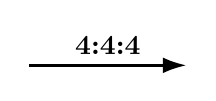
\begin{tikzpicture}
            \draw[-{Latex[length=3mm, width=2mm]}, line width=1pt] (0,0) -- (2,0) node[midway, above] {\textbf{4:4:4}};
        \end{tikzpicture}
    \end{minipage}
    \begin{minipage}[t]{0.25\textwidth}
        \centering
        \includegraphics[width=4.7cm,height=1.76cm]{cbcr.png}
    \end{minipage}
    
    \vspace{.6cm}
    
    \noindent
    \begin{minipage}[t]{0.25\textwidth}
        \centering
        \includegraphics[width=4.7cm,height=1.76cm]{cbcr.png}
    \end{minipage}
    \hspace{.24cm}
    \begin{minipage}[t]{0.2\textwidth}
        \centering
        \vspace{-1.3cm}
        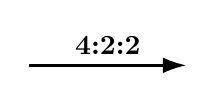
\begin{tikzpicture}
            \draw[-{Latex[length=3mm, width=2mm]}, line width=1pt] (0,0) -- (2,0) node[midway, above] {\textbf{4:2:2}};
        \end{tikzpicture}
    \end{minipage}
    \begin{minipage}[t]{0.25\textwidth}
        \centering
        \includegraphics[width=2.35cm,height=1.76cm]{cbcr.png}
    \end{minipage}
    
    \vspace{.6cm}
    
    \noindent
    \begin{minipage}[t]{0.25\textwidth}
        \centering
        \includegraphics[width=4.7cm,height=1.76cm]{cbcr.png}
    \end{minipage}
    \hspace{.24cm}
    \begin{minipage}[t]{0.2\textwidth}
        \centering
        \vspace{-1.3cm}
        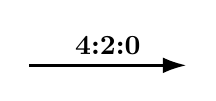
\begin{tikzpicture}
            \draw[-{Latex[length=3mm, width=2mm]}, line width=1pt] (0,0) -- (2,0) node[midway, above] {\textbf{4:2:0}};
        \end{tikzpicture}
    \end{minipage}
    \begin{minipage}[t]{0.25\textwidth}
        \centering
        \vspace{-1.2cm}
        \includegraphics[width=2.35cm,height=0.88cm]{cbcr.png}
    \end{minipage}

\end{center}


\subsection{Découpage en matrices 8$\times$8}
Les étapes suivantes sont réalisées sur les sous-blocs de taille 8$\times$8 des trois matrices (Y, Cb et Cr).



\begin{figure}[htbp]
    \centering
    \begin{subfigure}[b]{0.3\textwidth}
        \centering
        \includegraphics[width=.6\linewidth]{bloc_88.png}
        \caption*{\centering Une matrice 8$\times$8 extraite de la matrice de luminance}
    \end{subfigure}
    \hspace{1cm}
    \begin{subfigure}[b]{0.3\textwidth}
        \centering
        \includegraphics[width=.6\linewidth]{mat88_genere_aleatoirement.png}
        \caption*{\centering Une matrice 8x8 générée aléatoirement}
    \end{subfigure}
    % \caption{Caption globale pour les deux images}
\end{figure}

Il n'y a aucune redondance d'information à exploiter d'une matrice générée aléatoirement, mais les matrices 8$\times$8 considérées sont loin d'être aléatoires. Elles admettent une redondance sous la forme de fréquences spatiales que la transformée en cosinus discrète permet d'exploiter.


\subsection{Transformée en cosinus discrète}

La transformée en cosinus discrète (DCT) est similaire à la transformation de Fourier discrète : à un signal discret $(x_0,  \ldots, x_{N-1})$ elle associe les amplitudes de vecteurs d'une base fréquentielle.

\vspace{.2cm}

\begin{mydefinition}{Définition 1}
    La \textbf{DCT unidimensionnelle} est un endomorphisme \[\text{DCT} : \mathbb{R}^N \rightarrow \mathbb{R}^N, \quad (x_0, \ldots, x_{N-1}) \mapsto (X_0, \ldots, X_{N-1})\]

    \vspace{-0.1cm}
    \begin{equation*}
        \text{tel que } \quad X_k = \sqrt{\dfrac{2}{N}}c(k)\sum_{n=0}^{N-1} x_n \cos \left( \frac{k\pi}{N} \left( n + \frac{1}{2} \right) \right)
    \end{equation*}
    \[
        \text{avec} \ \ \ \ c(\alpha) =
        \begin{cases}
            \frac{1}{\sqrt{2}} & \text{si } \alpha = 0 \\
            1 & \text{sinon}
        \end{cases}
    \]
\end{mydefinition}




Voici un exemple :

\begin{figure}[H]
    \centering
    \includegraphics[width=0.5\linewidth]{uni.png}
\end{figure}

\begin{mydefinition}{Théorème 1}
    \textbf{La DCT est orthonormale}, c'est-à-dire que $\forall k, l \in \{0, 1, ..., N-1\}$,
    $$
    \dfrac{2}{N} c(k)c(l)\sum_{n=0}^{N-1} \cos \left( \frac{k\pi}{N} \left( n + \frac{1}{2} \right) \right)\cos \left( \frac{l\pi}{N} \left( n + \frac{1}{2} \right) \right) = \delta_{kl}
    $$
\end{mydefinition}

\begin{mydefinition}{Théorème 2}
    \textbf{La DCT conserve l'énergie du signal}, c'est-à-dire que $E_x = E_X$ 
    \[ \text{avec } \quad E_x = \sum_{n=0}^{N-1} x_n^2 \quad \text{ et } \quad E_X = \sum_{k=0}^{N-1} X_k^2 \]
    
\end{mydefinition}
    
    

Manipulant des images, la compression JPEG utilise la DCT bidimensionnelle que l'on peut déduire de la DCT unidimensionnelle en réalisant la DCT unidimensionnelle successivement sur les lignes puis sur les colonnes.

\vspace{0.2cm}

\begin{mydefinition}{Definition 2}
    La \textbf{DCT bidimensionnelle} est un endomorphisme \[\text{DCT} : \mathcal{M}_{N,N}(\mathbb{R}) \rightarrow \mathcal{M}_{N,N}(\mathbb{R}), \quad pixel \mapsto D \]
    
    \[
        \text{tel que} \quad D(i,j) = \frac{2}{N} c(i) c(j) \sum_{x=0}^{N-1} \sum_{y=0}^{N-1} pixel(x,y) \cos \left( \frac{\pi}{N} i \left( x + \frac{1}{2} \right) \right) \cos \left( \frac{\pi}{N} j \left( y + \frac{1}{2} \right) \right)
    \]
\end{mydefinition}

En pratique, dans la compression JPEG : \[\text{DCT} : \mathcal{M}_{8,8}(\{-128, -127, \ldots, 127\}) \rightarrow \mathcal{M}_{8,8}([-2048, 2048])\]

En effet, $Im(DCT) \subset \mathcal{M}_{8,8}([-2048, 2048]) $ car

\[
\left| D(i, j)\right| \leq \frac{1}{4}\left| \sum_{x=0}^{7} \sum_{y=0}^{7} pixel(x, y) \cos(...) \cos(...) \right| \leq \frac{1}{4} \sum_{x=0}^{7} \sum_{y=0}^{7} \left| pixel(x, y) \right| \leq \frac{1}{4} \cdot 64 \cdot 128 = 2048
\]


\vspace{0.2cm}

\begin{myproof}
    
    \textbf{Démonstration du passage de la DCT unidimensionnelle à la DCT bidimensionnelle} :
    
    \vspace{.25cm}

    Soit $pixel \in \mathcal{M}_{N,N}(\mathbb{R})$. On considère les indices de la matrice comme allant de 0 à $N-1$.

    \vspace{.2cm}
    
    Appliquons la DCT unidimensionnelle à chaque ligne $x$ de la matrice $pixel(x, y)$, en fixant $x$, et en sommant sur $y$ :
    
    $$
    F(x, j) = \sqrt{\dfrac{2}{N}} c(j) \sum_{y=0}^{N-1} pixel(x, y) \cos\left( \frac{j\pi}{N} \left( y + \frac{1}{2} \right) \right)
    $$
    
    Appliquons ensuite la DCT unidimensionnelle à chaque colonne $j$ de la matrice $F(x, j)$, en sommant cette fois sur $x$ :
    
    $$
    D(i, j) = \sqrt{\dfrac{2}{N}} c(i) \sum_{x=0}^{N-1} F(x, j) \cos\left( \frac{i\pi}{N} \left( x + \frac{1}{2} \right) \right)
    $$
    
    Remplaçons $F(x, j)$ dans cette expression :
    
    $$
    D(i, j) = \sqrt{\dfrac{2}{N}}c(i) \sum_{x=0}^{N-1} \left[\sqrt{\dfrac{2}{N}} c(j) \sum_{y=0}^{N-1} pixel(x, y) \cos\left( \frac{j\pi}{N} \left( y + \frac{1}{2} \right) \right) \right] \cos\left( \frac{i\pi}{N} \left( x + \frac{1}{2} \right) \right)
    $$
    
    Simplifions l’expression en regroupant les sommes doubles :
    
    $$
    D(i, j) = \frac{2}{N} c(i)c(j) \sum_{x=0}^{N-1} \sum_{y=0}^{N-1} pixel(x, y) \cos\left( \frac{i\pi}{N} \left( x + \frac{1}{2} \right) \right) \cos\left( \frac{j\pi}{N} \left( y + \frac{1}{2} \right) \right)
    $$

\end{myproof}

On peut visualiser les vecteurs de la base de la DCT. Les basses fréquences se trouvent en haut à gauche tandis que les hautes fréquences se trouvent en bas à droite.

\begin{figure}[H]
    \centering
    \includegraphics[width=.3\linewidth]{base_dct.png}
    \caption{Base de la DCT}
\end{figure}

Voici un exemple d'une matrice 8$\times$8 extraite décomposée dans la base canonique et dans la base DCT :

\hfill
\begin{minipage}{0.3\textwidth}
    \centering
    \begin{figure}[H]
        \centering
        \includegraphics[width=0.7\linewidth]{bloc_88.png}
        \caption*{\centering Une matrice 8x8}
    \end{figure}
\end{minipage}
\hfill
\begin{minipage}{0.3\textwidth}
    \centering
    \begin{table}[H]
        \setlength{\tabcolsep}{2pt}
        \renewcommand{\arraystretch}{1.2} % Ajuste l'espace entre les lignes

        \centering
        \begin{tabular}{cccccccc}
            160 & 156 & 153 & 147 & 140 & 134 & 127 & 108\\
            156 & 151 & 148 & 143 & 126 & 114 & 105 & 83\\
            153 & 144 & 138 & 140 & 117 & 97 & 82 & 61\\
            142 & 141 & 142 & 149 & 116 & 95 & 67 & 68\\
            126 & 120 & 124 & 121 & 102 & 65 & 65 & 68\\
            113 & 97 & 95 & 96 & 91 & 125 & 112 & 57\\
            102 & 100 & 95 & 90 & 98 & 121 & 140 & 122\\
            106 & 104 & 106 & 92 & 98 & 121 & 142 & 139\\
        \end{tabular}
        \caption*{Dans la base canonique}
    \end{table}
\end{minipage}
\hfill
\begin{minipage}{0.3\textwidth}
    \centering
    \begin{table}[H]
        \setlength{\tabcolsep}{2pt}
        \renewcommand{\arraystretch}{1.2} % Ajuste l'espace entre les lignes

        \centering
        \begin{tabular}{cccccccc}
            -99 & 98 & -20 & 20 & -16 & 20 & 2 & -6\\
            78 & 103 & -38 & -8 & 17 & -3 & -3 & -1\\
            58 & -75 & 40 & 0 & -13 & 1 & -8 & 13\\
            -7 & -18 & -4 & 23 & -14 & 5 & 4 & -2\\
            21 & 7 & -2 & -20 & 12 & -12 & 9 & -3\\
            12 & -10 & 1 & -2 & 2 & 0 & -6 & 0\\
            -9 & 4 & -3 & 15 & -7 & 8 & 0 & 0\\
            -2 & -2 & 6 & -5 & 5 & -7 & 2 & 1\\
        \end{tabular}
        \caption*{Dans la base DCT}
    \end{table}
\end{minipage}
\hfill



\subsection{Quantification}

L'objectif est de réduire la taille de l'information en approximant les basses fréquences (de manière à pouvoir les stocker sur moins de bits) et en éliminant les hautes fréquences (en les approximant par 0). Pour cela, la matrice de fréquence est divisée par une matrice de quantification coefficient par coefficient. On approxime chaque coefficient obtenu à l'entier le plus proche.

\textbf{k} est le facteur de quantification. On multiplie la matrice de fréquence par \textbf{k} afin de choisir le taux de compression. Plus \textbf{k} est petit plus la qualité est mauvaise et la taille de l'image compréssée est petite.

\vspace{17pt}

Voici un exemple avec \textbf{k} = 1 :

\vspace{.2cm}

\begin{minipage}{0.29\textwidth}
    \centering
    \begin{table}[H]
        \centering
        \setlength{\tabcolsep}{2pt} % Réduire l'espace entre les colonnes
        \renewcommand{\arraystretch}{1.2} % Ajuste l'espace entre les lignes

        \begin{tabular}{cccccccc}
            -99 & 98 & -20 & 20 & -16 & 20 & 2 & -6\\
            78 & 103 & -38 & -8 & 17 & -3 & -3 & -1\\
            58 & -75 & 40 & 0 & -13 & 1 & -8 & 13\\
            -7 & -18 & -4 & 23 & -14 & 5 & 4 & -2\\
            21 & 7 & -2 & -20 & 12 & -12 & 9 & -3\\
            12 & -10 & 1 & -2 & 2 & 0 & -6 & 0\\
            -9 & 4 & -3 & 15 & -7 & 8 & 0 & 0\\
            -2 & -2 & 6 & -5 & 5 & -7 & 2 & 1\\
        \end{tabular}
        \caption*{\centering matrice de fréquence \\ \ }
    \end{table}
\end{minipage}
\hfill
\begin{minipage}{0.09\textwidth}
    \centering
    \LARGE
    \vspace{-25pt}
    $ \textbf{$\cdot$ k $\div$} $
\end{minipage}
\hfill
\begin{minipage}{0.3\textwidth}
    \centering
    \begin{table}[H]
        \centering
        \setlength{\tabcolsep}{2pt} % Réduire l'espace entre les colonnes
        \renewcommand{\arraystretch}{1.2} % Ajuste l'espace entre les lignes
        \begin{tabular}{cccccccc}
            16 & 11 & 10 & 16 & 24 & 40 & 51 & 61\\
            12 & 12 & 14 & 19 & 26 & 58 & 60 & 55\\
            14 & 13 & 16 & 24 & 40 & 57 & 69 & 56\\
            14 & 17 & 22 & 29 & 51 & 87 & 80 & 62\\
            18 & 22 & 37 & 56 & 68 & 109 & 103 & 77\\
            24 & 35 & 55 & 64 & 81 & 104 & 113 & 92\\
            49 & 64 & 78 & 87 & 103 & 121 & 120 & 101\\
            72 & 92 & 95 & 98 & 112 & 100 & 103 & 99\\
        \end{tabular}
        \caption*{\centering matrice de quantification choisie empiriquement par JPEG}
    \end{table}
\end{minipage}
\hfill
\begin{minipage}{0.03\textwidth}
    \centering
    \LARGE
    \vspace{-25pt}
    \textbf{=}
\end{minipage}
\hfill
\begin{minipage}{0.23\textwidth}
    \centering
    \begin{table}[H]
        \centering
        \setlength{\tabcolsep}{3pt} % Réduire l'espace entre les colonnes
        \renewcommand{\arraystretch}{1.2} % Ajuste l'espace entre les lignes
        \begin{tabular}{cccccccc}
            -6 & 9 & -2 & 1 & -1 & 0 & 0 & 0 \\
            6 & 9 & -3 & 0 & 1 & 0 & 0 & 0 \\
            4 & -6 & 2 & 0 & 0 & 0 & 0 & 0 \\
            0 & -1 & 0 & 1 & 0 & 0 & 0 & 0 \\
            1 & 0 & 0 & 0 & 0 & 0 & 0 & 0 \\
            0 & 0 & 0 & 0 & 0 & 0 & 0 & 0 \\
            0 & 0 & 0 & 0 & 0 & 0 & 0 & 0 \\
            0 & 0 & 0 & 0 & 0 & 0 & 0 & 0 \\
        \end{tabular}
        \caption*{\centering Matrice quantifiée \\ \ }
    \end{table}
\end{minipage}

\vspace{.7cm}

On exploite encore une limite physiologique de l’œil humain dans le choix de la matrice de quantification (ci-dessus celle choisie par JPEG). L’œil humain n'est pas capable de discerner les hautes fréquences, il est beaucoup plus sensible aux informations des basses fréquences. La matrice de quantification est donc choisie avec des coefficient plus importants en bas à droite que en haut à gauche, afin de compresser davantage les hautes fréquences.

\subsection{Codage RLE et Huffman}

L'objectif est de coder la matrice quantifié en une suite de 0 et de 1.

\vspace{.3cm}

On réalise d'abord un parcours en zig zag de la matrice quatifié afin d'obtenir une liste où les basses fréquences se trouvent en début de liste et les hautes fréquences en fin de liste.

\vspace{.5cm}


\begin{minipage}{0.3\textwidth}
    \begin{figure}[H]
        \centering
        \includegraphics[width=0.9\linewidth]{zigzag.png}
        \caption{le parcours en zig zag}
    \end{figure}
\end{minipage}
\hfill
\begin{minipage}{0.65\textwidth}

    \vspace{.3cm}
    \begin{center}
        Voici un exemple :
    \end{center}
    \vspace{-.3cm}

    \hfill
    \begin{minipage}{0.45\textwidth}
        \centering
        \begin{table}[H]
            \centering
            \setlength{\tabcolsep}{3pt} % Réduire l'espace entre les colonnes
            \renewcommand{\arraystretch}{1.2} % Ajuste l'espace entre les lignes
            \begin{tabular}{cccccccc}
                -6 & 9 & -2 & 1 & -1 & 0 & 0 & 0 \\
                6 & 9 & -3 & 0 & 1 & 0 & 0 & 0 \\
                4 & -6 & 2 & 0 & 0 & 0 & 0 & 0 \\
                0 & -1 & 0 & 1 & 0 & 0 & 0 & 0 \\
                1 & 0 & 0 & 0 & 0 & 0 & 0 & 0 \\
                0 & 0 & 0 & 0 & 0 & 0 & 0 & 0 \\
                0 & 0 & 0 & 0 & 0 & 0 & 0 & 0 \\
                0 & 0 & 0 & 0 & 0 & 0 & 0 & 0 \\
            \end{tabular}
            \caption*{\centering Matrice quantifiée}
        \end{table}
    \end{minipage}
    \hfill
    \begin{minipage}{0.53\textwidth}
        \centering
        liste après zig zag : \\ -6, 9, 6, 4, 9, -2, 1, -3, -6, 0, 1, -1, 2, 0, -1, 0, 1, 0, 0, 0, 0, 0, 0, 0, 1, EOB
    \end{minipage}
    \hfill
\end{minipage}

\vspace{1cm}

\hfill
\begin{minipage}{0.47\textwidth}
    On applique ensuite un codage RLE (Run Length Encoding) où chaque coefficient non nul est mis sous la forme : ( 0-tête / catégorie ) [position]
    \begin{itemize}
        \item 0-tête : nombre des zéros qui le séparent de son prédecesseur non-nul 
        \item catégorie : catégorie du coefficient
        \item position : position dans la catégorie
    \end{itemize}
\end{minipage}
\hfill
\begin{minipage}{0.43\textwidth}
    \begin{figure}[H]
        \centering
        \includegraphics[width=1\linewidth]{categorie.png}
        \caption{Table des catégories}
    \end{figure}
\end{minipage}
\hfill

\vspace{.8cm} 

L'algorithme de Huffman est ensuite appliqué au éléments entre parenthèses, sans construire l'arbre de Huffman à partir des données (ce qui obligerait à stocker un arbre par matrice), mais en utilisant un arbre établi empiriquement par JPEG. La position est stockée en binaire sur le nombre de bit de la catégorie.

\vspace{.3cm} 

Voici un exemple :

\vspace{.3cm} 

Liste après zig zag : -6, 9, 6, 4, 9, -2, 1, -3, -6, 0, 1, -1, 2, 0, -1, 0, 1, 0, 0, 0, 0, 0, 0, 0, 1, EOB 

\vspace{.3cm} 

Après codage RLE : (0,3) 1, (0,4) 9, (0,3) 6, (0,3) 4, (0,4) 9, (0,2) 1, (0,1) 1, (0,2) 0, (0,3) 1, (1,1) 1, (0,1) 0, (0,2) 2, (1,1) 0, (1,1) 1, (7,1) 1, (0,0) 

\vspace{.3cm} 

Après Huffman (les espaces ne sont mis que pour la lisibilité) : 100 001 1011 1001 100 110 100 100 1011 1001 01 01 00 1 01 00 100 001 1100 1 00 0 01 11 1100 0 1100 1 11111010 1 1010


\subsection{Décompression}

Les étapes sont simplement effectuées dans l'ordre opposé car chaque étape est inversible :
\begin{itemize}[noitemsep,nolistsep]
    \item Décompression de Huffman
    \item Déduction de la liste à partir du codage RLE
    \item Reconstruction de la matrice quantifiée
    \item Multiplication par la matrice de quantification
    \item Utilisation de la DCT-inverse
    \item Assemblage des matrices 8x8
    \item Sur-échantillonnage
    \item Transformation des couleurs de YCbCr vers RVB
\end{itemize}


\section{Analyse des performances en taille et en qualité}


\subsection{Objectif}
Mon objectif est d'élaborer une technique permettant de choisir le meilleur facteur de quantification pour chaque image, dans le cas où l'image est partagée sur Instagram. Je définis le meilleur facteur de quantification comme le plus petit facteur de quantification où la qualité de l'image compressée est presque indiscernable de l'originale. Pour le choisir, il faut être en mesure de pouvoir estimer cette différence de qualité sans intervention humaine, et savoir lorsque la qualité de l'image n'est plus satisfaisante. C'est pour cela que l'on va s'intéresser à des indices de qualité.

\subsection{Indice de qualité}

\begin{mydefinition}{Definition 3}

    La \textbf{REQM (Racine de l'Erreur Quadratique Moyenne)} est la distance pour la norme deux $\|\mathbf{.}\|_2$ entre image originale est image compressée.

    \[ \text{Notons } \quad \quad img : \text{l'image originale} \quad \quad imgd : \text{l'image compressée}\]
    
    \[
    \text{REQM} = \sqrt{\frac{1}{3np} \sum_{i=0}^{n-1} \sum_{j=0}^{p-1} \sum_{k=0}^{2} \left( \text{img}(i, j, k) - \text{imgd}(i, j, k) \right)^2}
    \]
\end{mydefinition}

\begin{mydefinition}{Definition 4}

    Le \textbf{PSSB (rapport du Pic du Signal Sur Bruit)} est un indice de qualité s'appuyant sur la REQM, et allant de 0 (mauvaise qualité) à $+\infty$ (qualité parfaite).

    \[
    \text{PSSB} = 20 \cdot \log_{10} \left( \frac{255}{\text{REQM}} \right)
    \]
    
\end{mydefinition}

Cependant le PSSB calcule la qualité d'une image pixel par pixel, cette métrique est peu corrélée à la perception visuelle. L’œil humain est sensible à la structure, au contraste et à la luminance d'une image.

\begin{mydefinition}{Definition 5}

    Le \textbf{SSIM (Structural SIMilarity)} est un indice de qualité prenant en compte la luminance, le contraste et la structure des images originale et compressée, et allant de -1 (mauvaise qualité) à 1 (qualité parfaite).
    
    \[
        \text{SSIM} = 
        \underbrace{\frac{(2\mu_x\mu_y + c_1)}{(\mu_x^2 + \mu_y^2 + c_1)}}_{\text{\normalsize luminance}}
        \times
        \underbrace{\frac{(2\sigma_x\sigma_y + c_2)}{(\sigma_x^2 + \sigma_y^2 + c_2)}}_{\text{\normalsize contraste}}
        \times
        \underbrace{\frac{(\text{cov}_{xy} + c_3)}{(\sigma_x\sigma_y + c_3)}}_{\text{\normalsize structure}}
    \]

    \[
        \text{avec} \ 
        \begin{cases}
        \text{$x$ et $y$ deux matrices} \\
        \text{$\mu_x$ la moyenne de $x$, $\mu_y$ la moyenne de $y$} \\
        \text{$\sigma_x^2$ la variance de $x$, $\sigma_y^2$ la variance de $y$} \\
        \text{$\text{cov}_{xy}$ la covariance de $x$ et $y$} \\        
        \text{$c_1 = 6.5$, $c_2 = 58.5$ et $c_3 = 29.2$} \\        
        \end{cases}
    \]
    
\end{mydefinition}


Pour calculer le SSIM d'une image, on considère sa matrice de luminance et on calcule le SSIM de ses sous-blocs d'une certaine taille (par exemple les sous-blocs de taile 8$\times$8) puis on fait la moyenne de tout les SSIM.

\vspace{.3cm}

$c_1$, $c_2$ et $c_3$ sont choisis pour stabiliser la division lorsque les dénominateurs sont proches de 0.
\begin{itemize}[noitemsep,nolistsep]
    \item $c_1 = (k_1 L)^2$, $c_2 = (k_2 L)^2$ et $c_3 = \frac{c_2}{2}$
    \item $L$ : la dynamique des valeurs des pixels (255).
    \item $k_1 = 0,01$ et $k_2 = 0,03$ : des petites valeurs.
\end{itemize}


\subsection{Procédure expérimentale}

Ayant codé la compression JPEG en python, j'ai compressé 46 photos avec 11 facteurs de quantification différents. J'ai appliqué à chaque fois un sous-échantillonnage 4:2:0 et j'ai choisi comme matrice de quantification celle donnée par JPEG, il n'y a donc que l'évolution du facteur de quantification que j'analyse. J'ai ensuite calculé le PSSB et le SSIM des $46 \cdot 11 = 506$ photos compressées obtenues, ainsi que le rapport entre la taille de l'image compressée et la taille de l'image originale sans compression.

De plus, pour chacune des 46 photos, en faisant défiler devant mes yeux l'image de plus en plus compressée, j'ai pointé le dernier facteur de quantification tel que la qualité de l'image était encore satisfaisante (c'est-à-dire le meilleur facteur de quantification). Ces facteurs de quantification que j'ai pointés correspondent aux points noirs.

\subsection{Résultats de l'expérience}

Les résultats sont mis en forme dans le graphe suivant. Un trait représente une même image compressée avec 11 facteurs différents. Les indices de qualités fonctionnent bien pour une même image puisque plus l'image est compressée (et donc plus sa qualité est basse) plus l'indice de qualité diminue. 

Tous les facteurs de quantification que j'ai pointés (et qui représentent une qualité satisfaisante) ont une taille inférieure à 10 fois plus petite que l'image sans compression. Les 600 To estimés durant l'introduction peuvent donc être réduits à moins de 60 To.

Les points noirs représentant à mes yeux tous une même qualité, ils devraient être tous répartis sur la même ordonnée. Ceci n'étant le cas pour aucun des deux indices de qualité, on peut en déduire qu'ils ne donnent pas une valeur absolue de qualité, mais servent seulement à comparer une même image. Ils ne sont donc pas utilisables pour définir automatiquement le facteur de quantification adapté à chaque image.

Cependant, les facteurs de quantification que j'ai pointés sont très corrélés avec le facteur 1 affiché en rouge sur le graphique suivant. Ainsi, dans mon étude, il semble que le meilleur facteur de quantification à choisir est presque le même pour toute image : c'est le facteur 1.

\begin{figure}[H]
    \centering
    \includegraphics[width=0.7\linewidth]{graphe2.png}
    \caption{Les points noirs correspondent aux facteurs de quantification que j'ai pointés}
\end{figure}


\begin{figure}[H]
    \centering
    \includegraphics[width=0.7\linewidth]{graphe3.png}
    \caption{Les points rouges correspondent au facteur de quantification 1}
\end{figure}


\section{Bibliographie}
\ 

[1] Andrew B. Watson, Image Compression Using the Discrete Cosine Transform, Mathematica Journal, 4(1), 1994, p. 81-88 DOI:10.1007/978-3-322-96658-2 http://sites.apam.columbia.edu/courses/ap1601y/Watson\_MathJour\_94.pdf

\vspace{.4cm}

[2] TRINITY COLLEGE DUBLIN : introduction to the digital signal processing algorithms : \\ https://github.com/frcs/EE4C08

\vspace{.4cm}

[3] JOINT PHOTOGRAPHIC EXPERTS GROUP : Digital Compression and Coding of Continuous-tone Still images : https://www.w3.org/Graphics/JPEG/itu-t81.pdf

\vspace{.4cm}

[4] N. Ahmed, T.Natarajan, and K. R. Rao, “Discrete cosine transform,” IEEE Transactions on Computers, vol. C-32, pp. 90-93, Jan. 1974. doi:10.1109/t-c.1974.223784

\vspace{.4cm}

[5] ZHOU WANG; A.C. BOVIK; H.R. SHEIKH; E.P. SIMONCELLI : Image quality assessment: from error visibility to structural similarity : https://www.cns.nyu.edu/pub/lcv/wang03-preprint.pdf

\section{Annexes\label{annexe}}


\begin{mydefinition}{Lemme 1}
    \[
    \sum_{n=0}^{N-1} \cos\left(\frac{2k\pi}{N} \left(n + \frac{1}{2} \right)\right) = 0 \quad \text{si } k \neq 0.
    \]
\end{mydefinition}



\begin{myproof}
    \textbf{Démonstration du Lemme 1}

    En utilisant la formule d'Euler :
    
    \[
    \sum_{n=0}^{N-1} \cos\left(\frac{2k\pi}{N} \left(n + \frac{1}{2} \right)\right) 
    = \frac{1}{2} \sum_{n=0}^{N-1} \left( e^{i\frac{2k\pi}{N}(n + \frac{1}{2})} + e^{-i\frac{2k\pi}{N}(n + \frac{1}{2})} \right)
    \]
    
    \[
    =\frac{1}{2} \left( e^{i\theta/2} \sum_{n=0}^{N-1} e^{i\theta n} + e^{-i\theta/2} \sum_{n=0}^{N-1} e^{-i\theta n} \right) \quad \text{avec } \theta = \frac{2k\pi}{N} .
    \]
    
    
    On reconnaît une somme géométrique et \( e^{i\theta} \neq 1 \) donc
    
    \[
    \sum_{n=0}^{N-1} e^{i\theta n} = \frac{1 - e^{i\theta N}}{1 - e^{i\theta}} = \frac{1 - 1}{1 - e^{i\theta}} = 0 \quad \text{car } \theta N = 2k\pi
    \]
    
    
    On en déduit :
    \[
    \sum_{n=0}^{N-1} \cos\left(\frac{2k\pi}{N} \left(n + \frac{1}{2} \right)\right)
    = \frac{1}{2} \left( e^{i\theta/2} \cdot 0 + e^{-i\theta/2} \cdot 0 \right)
    = 0.
    \]

\end{myproof}


\begin{myproof}
    \textbf{Démonstration du Théorème 1}

    \ \ 
    
    \textbf{Démonstration de l'orthogonalité} : pour \( k \neq l \), En utilisant l'identité trigonométrique :
    \[
    \cos A \cos B = \frac{1}{2} \left[ \cos(A - B) + \cos(A + B) \right]
    \]
    
    on obtient :
    
    \[
    \sum_{n=0}^{N-1} \cos \left( \frac{k\pi}{N} \left( n + \frac{1}{2} \right) \right)\cos \left( \frac{l\pi}{N} \left( n + \frac{1}{2} \right) \right)
    \]
    
    \[
    = \frac{1}{2} \left[ \sum_{n=0}^{N-1} \cos\left( \frac{(k - l)\pi}{N}(n + \tfrac{1}{2}) \right) + \sum_{n=0}^{N-1} \cos\left( \frac{(k + l)\pi}{N}(n + \tfrac{1}{2}) \right) \right]
    \]
    
    \[
    = \frac{1}{2} \left[ 0 + 0 \right] = 0 \quad \text{d'après le \textbf{Lemme 1}}
    \]
    
    \vspace{.7cm}
    
    \textbf{Démonstration de l'othonormalité} : montrons que $\forall k \in \{0, 1, ..., N-1\}$
    $$
    \dfrac{2}{N} c(k)^2 \sum_{n=0}^{N-1} \cos^2\left(\frac{k\pi}{N} \left(n + \frac{1}{2} \right)\right) = 1
    $$

    \textbf{Étape 1} : Suppression du carré
    
    En utilisant l'identité trigonométrique :
    
    $$
    \cos^2 x = \frac{1 + \cos(2x)}{2}
    $$
    
    on obtient :
    
    $$
    \sum_{n=0}^{N-1} \cos^2\left(\frac{k\pi}{N} \left(n + \frac{1}{2} \right)\right) = \sum_{n=0}^{N-1} \left( \frac{1}{2} + \frac{1}{2} \cos\left(\frac{2k\pi}{N} \left(n + \frac{1}{2} \right)\right) \right)
    $$
    
    $$
    = \frac{N}{2} + \frac{1}{2} \sum_{n=0}^{N-1} \cos\left(\frac{2k\pi}{N} \left(n + \frac{1}{2} \right)\right)
    $$

    \textbf{Étape 2} : Calcul de la somme de cosinus


    si $k = 0$ :
    
    $$
    \sum_{n=0}^{N-1} \cos^2\left(0\right) = \sum_{n=0}^{N-1} 1 = N
    $$
    
    si $k \neq 0$ :
    
    $$
    \sum_{n=0}^{N-1} \cos\left(\frac{2k\pi}{N} \left(n + \frac{1}{2} \right)\right) = 0 \quad \text{d'après le \textbf{Lemme 1}}
    $$
    
    
    \textbf{Étape 3} : Calcul final
    
    si $k = 0$ : $$ \frac{2}{N} \cdot \frac{1}{2} \left(\frac{N}{2} + \frac{1}{2} \cdot N \right) = 1 $$
    
    si $k \neq 0$ : $$ X_k = \dfrac{2}{N} \cdot 1 \cdot \left(\frac{N}{2} + 0 \right) = 1 $$

    \vspace{.7cm}
    
    \textbf{Conclusion} : la DCT est bien orthonormale, on a bien que $\forall k, l \in \{0, 1, ..., N-1\}$ :
    $$\boxed{
    \dfrac{2}{N} c(k)c(l)\sum_{n=0}^{N-1} \cos \left( \frac{k\pi}{N} \left( n + \frac{1}{2} \right) \right)\cos \left( \frac{l\pi}{N} \left( n + \frac{1}{2} \right) \right) = \delta_{kl}
    }$$

\end{myproof}

\begin{myproof}
    \textbf{Démonstration du Théorème 2}

    \ \ 

    C'est une conséquence directe du \textbf{Théorème 1}.
    \\ 
    
    La DCT est orthonormale donc si $DCT(x) = X$ alors $\|x\|_2 = \|X\|_2 $ donc $E_x = E_X$ 
    
    

\end{myproof}

\end{document}
